\begin{figure}[!htb]
  \centering
  \begin{subfigure}[b]{0.9\textwidth}
    \centering
    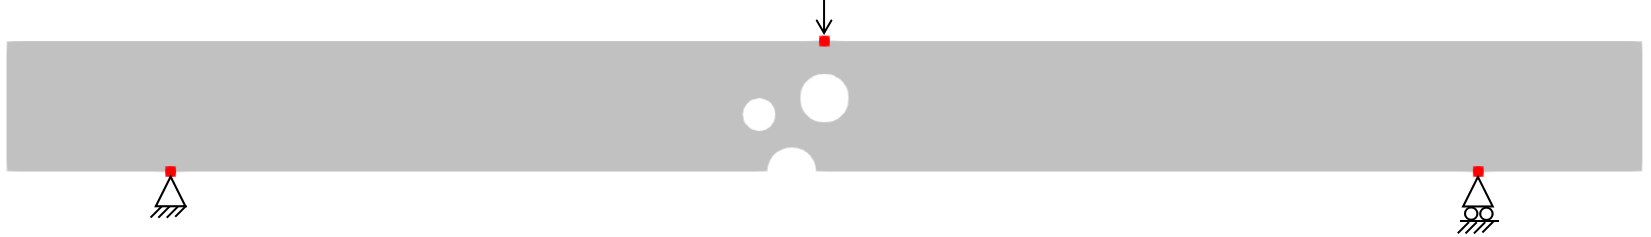
\includegraphics[width=\textwidth,scale=0.5]{Chapter5/figures/3pb/3pb_bc}
    \caption{}
  \end{subfigure}
  \begin{subfigure}[b]{0.9\textwidth}
    \centering
    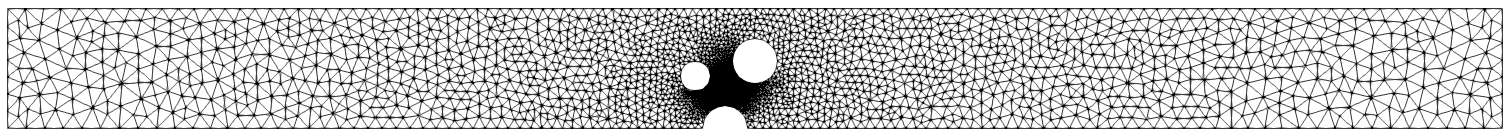
\includegraphics[width=\textwidth,scale=0.5]{Chapter5/figures/3pb/3pb_mesh}
    \caption{}
    \label{fig: Chapter5/3pb/3pb_mesh}
  \end{subfigure}
  \caption[Schematics of the three-point bending experiment and the mesh.]{(a) Schematics of the three-point bending experiment and (b) the mesh. See \cite{kubik2019ductile} for a detailed drawing with dimensions. The specimen is assumed to have a fixed support and a roller support on the bottom, and a downward displacement is applied at the location of the top punch.}
  \label{fig: Chapter5/3pb/3pb}
\end{figure}
